\begin{name}
	{Biên soạn: Thầy Trần Chiến, Bui Anh Tuan, Phan Anh}
	{Đề thi thử lần 1 THPT chuyên Thoại Ngọc Hầu - An Giang, năm học 2020-2021}
\end{name}
	\setcounter{ex}{0}\setcounter{bt}{0}
	\Opensolutionfile{ans}[ans/ans-2-GHK1-24-ChuyenThoaiNgocHau-AnGiang-21]

\begin{ex}%[Đề giữa kì 1 THPT Chuyên Thoại Ngọc Hầu - An Giang - 21,EX3-24-Phan Anh]%[2D2Y4-1]
	Tìm tập xác định $\mathscr{D}$ của hàm số $y=(2x-3)^{\sqrt{2019}}$
	\choice
	{$\mathscr{D}=(0;+\infty)$}
	{\True $\mathscr{D}=\left(\dfrac{3}{2};+\infty\right)$}
	{$\mathscr{D}=\mathbb{R}\setminus\left\{\dfrac{3}{2}\right\}$}
	{$\mathscr{D}=\mathbb{R}$}
	\loigiai{Do $\sqrt{2019}\not\in\mathbb{Z}$ nên hàm số xác định khi và chỉ khi $2x-3>0\Leftrightarrow x>\dfrac{3}{2}$.\\
		Vậy tập xác định của hàm số là $\mathscr{D}=\left(\dfrac{3}{2};+\infty\right)$.}
\end{ex}
\begin{ex}%[Thi thử, Chuyên Thoại Ngọc Hầu, An Giang, lần 1 2021]%[Bùi Anh Tuấn, 12EX3]%[2D2Y4-3]
	Cho $a$ là số thực lớn hơn $1$. Khẳng định nào sau đây là đúng?
	\choice
	{Hàm số $y=\log_a x$ đồng biến trên $\mathbb{R}$}
	{Hàm số $y=\log_a x$ nghịch biến trên $\mathbb{R}$}
	{\True Hàm số $y=\log_a x$ đồng biến trên $(0;+\infty)$}
	{Hàm số $y=\log_a x$ nghịch biến trên $(0;+\infty)$}
	\loigiai{
		Ta có $y=\log_a x\Rightarrow y'=\dfrac{1}{x.\ln a}>0,\ \forall x>0, a>1$.\\
		Chứng tỏ hàm số đồng biến trên khoảng $(0;+\infty)$
	}
\end{ex}
\begin{ex}%[Thi thử, Chuyên Thoại Ngọc Hầu, An Giang, lần 1 2021]%[Bùi Anh Tuấn, 12EX3]%[2D2Y1-2]
	Rút gọn biểu thức $P=x^{\frac{1}{3}}\cdot \sqrt[6]{x}$ với $x>0$
	\choice
	{\True $P=\sqrt{x}$}
	{$P=x^{\frac{1}{3}}$}
	{$P=x^{\frac{1}{9}}$}
	{$P=x^2$}
	\loigiai{
		Ta có $P=x^{\tfrac{1}{3}}\cdot \sqrt[6]{x}=x^{\tfrac{1}{3}}\cdot x^{\tfrac{1}{6}}=x^{\tfrac{1}{2}}=\sqrt{x}$
	}
\end{ex}
\begin{ex}%[Đề giữa kì 1 THPT Chuyên Thoại Ngọc Hầu - An Giang - 21,EX3-24-Phan Anh]%[2D2Y6-1]
	Bất phương trình $\log_{\tfrac{1}{2}}(x-1)>1$ có tập nghiệm $S$ là
	\choice
	{\True $S=\left(1;\dfrac{3}{2}\right)$}
	{$S=\left[1;\dfrac{3}{2}\right)$}
	{$S=\left(-\infty;\dfrac{3}{2}\right)$}
	{$S=\left(\dfrac{3}{2};+\infty\right)$}
	\loigiai{Điều kiện: $x-1>0\Leftrightarrow x>1$.\\
		Bất phương trình đã cho tương đương với $x-1<\dfrac{1}{2}\Leftrightarrow x<\dfrac{3}{2}$.\\
		Vậy tập nghiệm của bất phương trình là $S=\left(1;\dfrac{3}{2}\right)$.}
\end{ex}
\begin{ex}%[Đề giữa kì 1 THPT Chuyên Thoại Ngọc Hầu - An Giang - 21,EX3-24-Phan Anh]%[2D2Y5-1]
	Nghiệm của phương trình $\log_2(1-x)=2$ là
	\choice
	{$x=-4$}
	{\True $x=-3$}
	{$x=3$}
	{$x=5$}
	\loigiai{Phương trình đã cho tương đương với $1-x=2^2=4\Leftrightarrow x=-3$.}
\end{ex}
\begin{ex}%[Thi thử, Chuyên Thoại Ngọc Hầu, An Giang, lần 1 2021]%[Bùi Anh Tuấn, 12EX3]%[2D1Y2-2]
	\immini{Cho hàm số $f(x)$ xác định, liên tục trên đoạn $[-2;2]$ và có đồ thị là đường cong trong hình vẽ bên. Hàm số $f(x)$ đạt cục đại tại điểm nào dưới đây?
		\choice
		{$x=-2$}
		{\True $x=-1$}
		{$x=1$}
		{$x=2$}}{\begin{tikzpicture}[scale=.6, font=\footnotesize, line join=round, line cap=round, >=stealth, x=1.35cm, y=1cm]
			\def\xmin{-3}\def\xmax{3}\def\ymin{-4}\def\ymax{4}
			\draw[->] (\xmin-0.2,0)--(\xmax+0.2,0) node[below] {\footnotesize $x$};
			\draw[->] (0,\ymin-0.2)--(0,\ymax+0.2) node[right] {\footnotesize $y$};
			\draw (0,0) node [below left] {\footnotesize $O$};
			\fill (0,0) circle (2pt);
			\draw (-2.5,0) node [below ] {\footnotesize $-2$};
			\draw (-1.0,0) node [below ] {\footnotesize $-1$};
			\draw (1.0,0) node [above ] {\footnotesize $1$};
			\draw (2.15,0) node [below] {\footnotesize $2$};
			\draw (0,-3.85) node [left] {\footnotesize $-4$};
			\draw (0,3.65) node [left] {\footnotesize $4$};
			\draw (0,-1.9) node [left] {\footnotesize $-2$};
			\draw (0,1.9) node [right] {\footnotesize $2$};
			\foreach \x in {}\draw (\x,0.1)--(\x,-0.1) node [below] {\footnotesize $\x$};
			\foreach \y in {}\draw (0.1,\y)--(-0.1,\y) node [left] {\footnotesize $\y$};
			\clip (\xmin,\ymin) rectangle (\xmax,\ymax);
			\draw[smooth,samples=200,domain=\xmin:\xmax] plot (\x,{1*((\x)^3)+0*((\x)^2)+-3*(\x)+0});
			\draw[dashed] (0.0,0)--(0.0,0.0)--(0,0.0);\fill (0.0,0.0) circle (1pt);
			\draw[dashed] (-2.15,0)--(-2.15,-3.5)--(0,-3.5);\fill (-2.15,-3.5) circle (1pt);
			\draw[dashed] (2.15,0)--(2.15,3.5)--(0,3.5);\fill (2.15,3.5) circle (1pt);
			\draw[dashed] (1.0,-2.0)--(0,-2.0);\fill (1.0,-2.0) circle (1pt);
			\draw[dashed] (-1.0,2.0)--(0,2.0);\fill (-1.0,2.0) circle (1pt);
			\draw[dashed] (1.0,-2.0)--(1,0);\fill (1.0,-2.0) circle (1pt);
			\draw[dashed] (-1.0,2.0)--(-1,0);\fill (1.0,-2.0) circle (1pt);
	\end{tikzpicture}}
	\loigiai{
		Dựa vào đồ thị ta thấy hàm số $f(x)$ đạt cực đại tại $x=-1$.
	}
\end{ex}
\begin{ex}%[Đề giữa kì 1 THPT Chuyên Thoại Ngọc Hầu - An Giang - 21,EX3-24-Phan Anh]%[2D1B1-1]
	Hàm số $y=2x^4+1$ đồng biến trên khoảng nào trong các khoảng sau?
	\choice
	{$\left(-\infty;-\dfrac{1}{2}\right)$}
	{$\left(-\dfrac{1}{2};+\infty\right)$}
	{$(-\infty;0)$}
	{\True $(0;+\infty)$}
	\loigiai{\immini{Ta có $y'=8x^3$, $y'=0\Leftrightarrow x=0$.\\
			Bảng biến thiên của hàm số như hình bên.\\
			Từ bảng biến thiên ta suy ra hàm số đồng biến trên $(0;+\infty)$.}
		{
\begin{tikzpicture}
				\tkzTabInit[nocadre=false, lgt=1.2, espcl=2.5, deltacl=0.6]
				{$x$/0.7, $y'$/0.7, $y$/1.8}
				{$-\infty$,$0$,$+\infty$}
				\tkzTabLine{,-,0,+,}
				\tkzTabVar{+/$+\infty$,-/$1$,+/$+\infty$}
	\end{tikzpicture}}}
\end{ex}
\begin{ex}%[Thi thử lần 1, THPT chuyên Thoại Ngọc Hầu - An Giang, năm 2020 - 2021]%[Trần Chiến, 12EX3]%[2H1Y3-2]
	Thể tích của khối lập phương có cạnh $2a$ bằng
	\choice
	{$a^3$}
	{$2a^3$}
	{$6a^3$}
	{\True $8a^3$}
	\loigiai{
		Thể tích của khối lập phương có cạnh $2a$ là $(2a)^3 = 8a^3$. 	
	}
\end{ex}
\begin{ex}%[Thi thử lần 1, THPT chuyên Thoại Ngọc Hầu - An Giang, năm 2020 - 2021]%[Trần Chiến, 12EX3]%[2D1Y1-2]
	\immini{
		Cho hàm số $f(x)$ có đồ thị như hình vẽ bên. Hàm số đã cho nghịch biến trên khoảng nào trong các khoảng sau?
		\choice
		{$(0;2)$}
		{$(-2;0)$}
		{$(-3;-1)$}
		{\True $(2;3)$}
	}{
		\begin{tikzpicture}[scale=0.73, font=\footnotesize, line join=round, line cap=round,>=stealth]
			\def\a{1} \def\b{1} \def\c{1} \def\d{-1} % Hệ số
			\def\xmin{-4} \def\xmax{4.5}
			\def\ymin{-3.7} \def\ymax{4}			
			\draw[->] (\xmin,0)--(\xmax,0) node [above]{$x$};
			\draw[->] (0,\ymin)--(0,\ymax) node [right]{$y$};
			\clip (\xmin+0.1,\ymin+0.1) rectangle (\xmax-0.1,\ymax-0.1);
			\draw[smooth,samples=300,domain=-3:1] plot(\x,{-(\x)^2-2*(\x)});
			\draw[smooth,samples=300,domain=1:3] plot(\x,{-6*(\x)^2+24*(\x)-21});
			\draw[dashed] (-3,0)--(-3,-3)--(3,-3)--(3,0)
			(-1,0)--(-1,1)--(0,1)
			(1,0)--(1,-3)
			(0,3)--(2,3)--(2,0);
			\fill (0,0) circle (1pt) node[below left]{$O$} 
			(-3,0) circle (1pt)node[above]{$-3$} 
			(-1,0) circle (1pt)node[below]{$-1$}
			(1,0) circle (1pt)node[above]{$1$}
			(3,0) circle (1pt)node[above]{$3$}
			(2,0) circle (1pt)node[below]{$2$}
			(0,1) circle (1pt)node[right]{$1$}
			(0,3) circle (1pt)node[left]{$3$}
			(0,-3) circle (1pt)node[below left]{$-3$}
			;
		\end{tikzpicture}
	}
	\loigiai{
		Dựa vào đồ thị suy ra hàm số nghịch biến trên khoảng $(2;3)$.	
	}
\end{ex}
\begin{ex}%[Thi thử, Chuyên Thoại Ngọc Hầu, An Giang, lần 1 2021]%[Bùi Anh Tuấn, 12EX3]%[2D1Y5-1]
	Trong bốn hàm số được liệt kê ở bốn phương án A, B, C, D dưới đây, hàm số nào có bảng biến thiên như sau?
	\begin{center}
		
\begin{tikzpicture}[>=stealth]
			\tkzTabInit[nocadre=false,lgt=1,espcl=2,deltacl=0.5]{$x$/.7 ,$y'$/.7,$y$/2}
			{$-\infty$ , $-1$ , $0$ , $1$ , $+\infty$}
			\tkzTabLine{ , + , $0$ , - , $0$ , + , $0$ , - , }
			\tkzTabVar{-/$-\infty$ , +/$3$, -/$2$ , +/$3$ , -/$-\infty$}
		\end{tikzpicture}
	\end{center}
	\choice
	{$y=x^4-2x^2+1$}
	{$y=-x^4+2x^2+1$}
	{$y=x^4-2x^2+2$}
	{\True $y=-x^4+2x^2+2$}
	\loigiai{
		Từ bảng biến thiên ta thấy đây là hàm trùng phương $y=ax^4+bx^2+c$ có hệ số $a<0$ (vì $\lim \limits_{x \to \pm \infty} y=-\infty$) và hệ số $c>0$ (vì đồ thị cắt trục tung tại điểm có tung độ dương là $y=2$).\\
		Mặt khác, đồ thị đã cho có ba điểm cực trị nên hệ số $b>0$. Do đó chỉ có hàm số $y=-x^4+2x^2+2$ trong bốn hàm số trên thỏa mãn.
	}
\end{ex}
\begin{ex}%[Thi thử, Chuyên Thoại Ngọc Hầu, An Giang, lần 1 2021]%[Bùi Anh Tuấn, 12EX3]%[2D1B5-4]
	Cho hàm số $ y=(x-2)(x^2+1) $ có đồ thị $ (C) $. Mệnh đề nào sau đây là đúng?
	\choice
	{$ (C) $ không cắt trục hoành}
	{\True $ (C) $ cắt trục hoành tại một điểm}
	{$ (C) $ cắt trục hoành tại hai điểm}
	{$ (C) $ cắt trục hoành tại ba điểm}
	\loigiai{
		Xét phương trình hoành độ giao điểm $ (x-2)(x^2+1)=0\Leftrightarrow x=2 $. Phương trình có $ 1 $ nghiệm nên $ (C) $ cắt trục hoành tại $ 1 $ điểm.
	}
\end{ex}
\begin{ex}%[Thi thử, Chuyên Thoại Ngọc Hầu, An Giang, lần 1 2021]%[Bùi Anh Tuấn, 12EX3]%[2D1B5-1]
	\immini{Đường cong ở hình bên là đồ thị của một trong bốn hàm số dưới đây. Hàm số đó là hàm số nào?
		\choice
		{\True $y=x^3-3x^2+3$}
		{$y=-x^4+2x^2+1$}
		{$y=x^4-2x^2+1$}
		{$y=-x^3+3x^2+1$}}
	{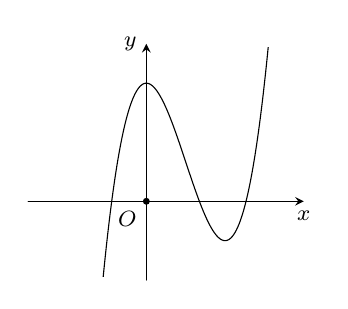
\begin{tikzpicture}[scale=0.5,>=stealth, font=\footnotesize, line join=round, line cap=round]
			\def\a{1} \def\b{-6} \def\c{9} \def\d{1} % Hệ số
			\def\xmin{-3} \def\xmax{4}
			\def\ymin{-2} \def\ymax{4} 
			%\draw[color=gray!50,dashed] (\xmin,\ymin) grid (\xmax,\ymax); 
			\draw[->] (\xmin,0)--(\xmax,0) node [below]{$x$};
			\draw[->] (0,\ymin)--(0,\ymax) node [left]{$y$};
			%\node at (0,0) [below left]{$O$};
			\fill (0,0)node[below left]{$O$}circle(2.5 pt);
			\clip (\xmin+0.1,\ymin+0.1) rectangle (\xmax-0.5,\ymax-0.1);
			\draw[smooth,samples=300] plot(\x,{(\x)^3-3*(\x)^2+3});
	\end{tikzpicture}}
	\loigiai{
		Ta thấy đây là đồ thị của hàm số bậc ba có hệ số $a>0$.\\
		Vậy hàm số cần tìm là $y=x^3-3x^2+3$.
	}
\end{ex}
\begin{ex}%[Đề giữa kì 1 THPT Chuyên Thoại Ngọc Hầu - An Giang - 21,EX3-24-Phan Anh]%[2D2Y4-2]
	Tính đạo hàm của hàm số $y=2^{x^2}$.
	\choice
	{$y'=2^x\cdot\ln2^x$}
	{\True $y'=x\cdot2^{1+x^2}\ln2$}
	{$y'=\dfrac{x\cdot2^{1+x^2}}{\ln2}$}
	{$y'=\dfrac{x\cdot2^{1+x}}{\ln2}$}
	\loigiai{Ta có $y'=\left(x^2\right)'\cdot2^{x^2}\ln2=2x\cdot2^{x^2}\ln2=x\cdot2^{1+x^2}\ln2$.}
\end{ex}
\begin{ex}%[Thi thử, Chuyên Thoại Ngọc Hầu, An Giang, lần 1 2021]%[Bùi Anh Tuấn, 12EX3]%[2D2B3-2]
	Cho $a$, $b$, $x$, $y$ là các số thực dương và $a$, $b$ khác $1$. Mệnh đề nào sau đây đúng?
	\choice
	{$\log _{a} \dfrac{x}{y}=\dfrac{\log _{a} x}{\log _{a} y}$}
	{$\log _{a} \dfrac{x}{y}=\log _{a}(x-y)$}
	{\True $\log _{b} a \cdot \log _{a} x=\log _{b} x$}
	{$\log _{a} x+\log _{a} y=\log _{a}(x+y)$}
	\loigiai{
		Ta có
		\begin{itemize}
			\item $\log _{a} \dfrac{x}{y}=\dfrac{\log _{a} x}{\log _{a} y}$ và $\log _{a} \dfrac{x}{y}=\log _{a}(x-y)$ là các mệnh đề sai vì $\log _{a} \dfrac{x}{y}=\log _{a} x-\log _{a} y$.
			\item $\log _{b} a \cdot \log _{a} x=\log _{b} x$ là mệnh đề đúng.
			\item $\log _{a} x+\log _{a} y=\log _{a}(x+y)$ là mệnh đề sai vì $\log _{a} x+\log _{a} y=\log _{a} (xy)$.
		\end{itemize}
	}
\end{ex}
\begin{ex}%[Thi thử, Chuyên Thoại Ngọc Hầu, An Giang, lần 1 2021]%[Bùi Anh Tuấn, 12EX3]%[2D2B1-3] 
	Tìm tập tất cả các giá trị của $a$ để  $\sqrt[15]{a^7}>\sqrt[5]{a^2}$.
	\choice
	{$a<0$}
	{$a=0$}
	{$0<a<1$}
	{\True $a>1$}
	\loigiai{
		Ta có $\sqrt[5]{a^2}=\sqrt[15]{a^6}$. Do đó $\sqrt[15]{a^7}>\sqrt[5]{a^2}\Leftrightarrow \sqrt[15]{a^7}>\sqrt[15]{a^6}
		$ mà $7>6$ nên $a>1$.
	}
\end{ex}
\begin{ex}%[Thi thử, Chuyên Thoại Ngọc Hầu, An Giang, lần 1 2021]%[Bùi Anh Tuấn, 12EX3]%[2H1B2-3]
	Hình lăng trụ tam giác đều có bao nhiêu mặt phẳng đối xứng?
	\choice
	{$1$}
	{$3$}
	{\True $4$}
	{$6$}
	\loigiai{
		Hình lăng trụ tam giác đều có $4$ mặt phẳng đối xứng gồm
		\begin{center}
			\begin{tikzpicture}[scale=.4]
				\tkzDefPoints{0/0/A, 1.5/-1/B, 5/0/C, 0/5/z}
				\coordinate (D) at ($(A)+(z)$);
				\coordinate (E) at ($(B)+(z)$);
				\coordinate (F) at ($(C)+(z)$);
				\coordinate (M) at ($(E)!0.5!(F)$);
				\coordinate (N) at ($(B)!0.5!(C)$);	
				\tkzDrawPolygon(E,F,D)
				\tkzFillPolygon[color=blue,fill opacity=0.5](A,D,M,N)
				\tkzDrawSegments(D,A A,B B,C B,E C,F)
				\tkzDrawSegments[dashed](A,C)
			\end{tikzpicture}
			\qquad
			\begin{tikzpicture}[scale=.4]
				\tkzDefPoints{0/0/A, 1.5/-1/B, 5/0/C, 0/5/z}
				\coordinate (D) at ($(A)+(z)$);
				\coordinate (E) at ($(B)+(z)$);
				\coordinate (F) at ($(C)+(z)$);
				\coordinate (M) at ($(D)!0.5!(E)$);
				\coordinate (N) at ($(A)!0.5!(B)$);	
				\tkzDrawPolygon(E,F,D)
				\tkzFillPolygon[color=red,fill opacity=0.5](C,F,M,N)
				\tkzDrawSegments(D,A A,B B,C B,E C,F)
				\tkzDrawSegments[dashed](A,C)
			\end{tikzpicture}
			\qquad	
			\begin{tikzpicture}[scale=.4]
				\tkzDefPoints{0/0/A, 1.5/-1/B, 5/0/C, 0/5/z}
				\coordinate (D) at ($(A)+(z)$);
				\coordinate (E) at ($(B)+(z)$);
				\coordinate (F) at ($(C)+(z)$);
				\coordinate (M) at ($(D)!0.5!(F)$);
				\coordinate (N) at ($(A)!0.5!(C)$);	
				\tkzDrawPolygon(E,F,D)
				\tkzFillPolygon[color=green,fill opacity=0.5](B,E,M,N)
				\tkzDrawSegments(D,A A,B B,C B,E C,F)
				\tkzDrawSegments[dashed](A,C)
			\end{tikzpicture}
			\qquad
			\begin{tikzpicture}[scale=.4]
				\tkzDefPoints{0/0/A, 1.5/-1/B, 5/0/C, 0/5/z}
				\coordinate (D) at ($(A)+(z)$);
				\coordinate (E) at ($(B)+(z)$);
				\coordinate (F) at ($(C)+(z)$);
				\coordinate (M) at ($(A)!0.5!(D)$);
				\coordinate (N) at ($(B)!0.5!(E)$);
				\coordinate (P) at ($(C)!0.5!(F)$);
				\tkzDrawPolygon(E,F,D)
				\tkzFillPolygon[color=yellow,fill opacity=0.5](M,N,P)
				\tkzDrawSegments(D,A A,B B,C B,E C,F)
				\tkzDrawSegments[dashed](A,C)
			\end{tikzpicture}
		\end{center}
	}
\end{ex}
\begin{ex}%[Thi thử lần 1, THPT chuyên Thoại Ngọc Hầu - An Giang, năm 2020 - 2021]%[Trần Chiến, 12EX3]%[2D1B3-1]
	Tìm giá trị lớn nhất của hàm số $f(x)= x^3-2x^2-4x+1$ trên đoạn $[1;3]$.
	\choice
	{$-7$}
	{$-4$}
	{\True $-2$}
	{$\dfrac{67}{27}$}
	\loigiai{
		Ta có $f'(x) = 3x^2-4x-4$; $f'(x) =0\Leftrightarrow \hoac{& x=2 \\ &x =-\dfrac{2}{3} \notin [1;3].}$
		\\
		Ta có $f(1) = -4; f(2)=-7 ; f(3) =-2 $. \\
		Vậy giá trị lớn nhất của hàm số trên đoạn $[1;3]$ là $-2$.	
	}
\end{ex}
\begin{ex}%[Thi thử lần 1, THPT chuyên Thoại Ngọc Hầu - An Giang, năm 2020 - 2021]%[Trần Chiến, 12EX3]%[2H1B3-2]
	Cho hình chóp $S.ABC$ có đáy $ABC$ là tam giác đều cạnh $a$, $SA$ vuông góc với mặt phẳng $(ABC)$, góc giữa đường thẳng $SB$ và mặt phẳng $(ABC)$ bằng $60^\circ$. Thể tích của khối chóp đã cho bằng
	\choice
	{$a^3$}
	{$\dfrac{a^3}{2}$}
	{\True $\dfrac{a^3}{4}$}
	{$\dfrac{3a^3}{4}$}
	\loigiai{
	\immini{	
	Do $\triangle ABC$ đều cạnh $a$ nên $S_{\triangle ABC}=\dfrac{a^2\sqrt{3}}{4}$.\\
	Do $SA$ vuông góc với $(ABC)$ tại $B$ nên $AB$ là hình chiếu của $SB$ xuống mặt phẳng $(ABC)$. Vì vậy, góc giữa đường thẳng $SB$ và đáy là góc $\widehat{SBA}$.\\
	Xét $\triangle SAB$ vuông tại $A$, ta có $SA=AB\cdot \tan 60=a\sqrt{3}$.\\
	Thể tích khối chóp đã cho là 
	\[V=\dfrac{1}{3}\cdot SA\cdot S_{\triangle ABC} =\dfrac{1}{3}\cdot a\sqrt{3} \cdot \dfrac{a^2\sqrt{3}}{4}= \dfrac{a^3}{4}.\]
	}{
	\begin{tikzpicture}[scale=1, font=\footnotesize, line join=round, line cap=round,>=stealth]
	\tkzDefPoints{0/0/A,3/0/C,1.5/-1/B}
	\coordinate (S) at ($(A)+(0,3)$);
	\tkzDrawSegments(S,A S,B S,C A,B B,C)
	\tkzDrawSegments[dashed](A,C)
	\tkzLabelPoints[above](S)
	\tkzLabelPoints[below left](A)
	\tkzLabelPoints[below right](C)
	\tkzLabelPoints[below](B)
	\tkzDrawPoints(S,A,B,C)
	\tkzMarkAngle[size=0.5](S,B,A)
	\end{tikzpicture}	
	}	
	}
\end{ex}

\begin{ex}%[Thi thử lần 1, THPT chuyên Thoại Ngọc Hầu - An Giang, năm 2020 - 2021]%[Trần Chiến, 12EX3]%[1D1B2-1]
	Hỏi trên $\left[0;\dfrac{\pi}{2}\right)$, phương trình $\sin x =\dfrac{1}{2}$ có bao nhiêu nghiệm?
	\choice
	{\True $1$}
	{$2$}
	{$3$}
	{$4$}
	\loigiai{
	Do hàm số $y=\sin x$ đồng biến trên $\left[0;\dfrac{\pi}{2}\right)$ nên phương trình $\sin x =\dfrac{1}{2}$ có duy nhất 1 nghiệm $x= \dfrac{\pi}{6}$ trên tập $\left[0;\dfrac{\pi}{2}\right)$.
	}
\end{ex}
\begin{ex}%[Đề giữa kì 1 THPT Chuyên Thoại Ngọc Hầu - An Giang - 21,EX3-24-Phan Anh]%[2H1B3-1]
	Cho hình bát diện đều cạnh $a$. Gọi $S$ là tổng diện tích tất cả các mặt của hình bát diện đó. Mệnh đề nào dưới đây đúng?
	\choice
	{$S=a^2\sqrt{3}$}
	{\True $S=2a^2\sqrt{3}$}
	{$S=4a^2\sqrt{3}$}
	{$S=8a^2$}
	\loigiai{Mỗi mặt của bát diện đều là tam giác đều, nên tổng diện tích các mặt của bát diện đều là
		$$S=8\cdot S_{\text{mặt}}=8\cdot\dfrac{a^2\sqrt{3}}{4}=2a^2\sqrt{3}.$$}
\end{ex}
\begin{ex}%[Thi thử lần 1, THPT chuyên Thoại Ngọc Hầu - An Giang, năm 2020 - 2021]%[Trần Chiến, 12EX3]%[2D1B2-1]
	Giá trị cực đại của hàm số $y= x^3-3x+2$ là
	\choice
	{$-1$}
	{$0$}
	{$1$}
	{\True $4$}
	\loigiai{
		Tập xác định $\mathscr{D}=\mathbb{R}$.\\
		Ta có $y' = 3x^2-3$ và $y'=0 \Leftrightarrow x=\pm 1$.\\
		Lại có $y'' = 6x$, suy ra $y''(1)=6>0$ và $y''(-1)=-6<0$.\\
		Vì vậy hàm số đạt cực đại tại $x=-1$ và $y_{\text{CĐ}} =y(-1)=4$.	
	}
\end{ex}
\begin{ex}%[Thi thử lần 1, THPT chuyên Thoại Ngọc Hầu - An Giang, năm 2020 - 2021]%[Trần Chiến, 12EX3]%[2H1B3-2]
	Cho hình chóp $S.ABCD$ có đáy $ABCD$ là hình vuông cạnh $a$, cạnh bên $SA$ vuông góc với đáy và $SA=a\sqrt{2}$. Thể tích của khối chóp đã cho bằng
	\choice
	{$a^3\sqrt{2}$}
	{\True $\dfrac{a^3\sqrt{2}}{3}$}
	{$\dfrac{a^3\sqrt{2}}{4}$}
	{$\dfrac{a^3\sqrt{2}}{6}$}
	\loigiai{
		\immini{
			Thể tích của khối chóp là \[V=\dfrac{1}{3}SA\cdot S_{ABCD}=\dfrac{1}{3}\cdot a\sqrt{2}\cdot a^2=\dfrac{a^3\sqrt{2}}{3}.\]
		}{
			\begin{tikzpicture}[scale=0.6, font=\footnotesize, line join=round, line cap=round,>=stealth]
				\tkzDefPoints{0/0/A,5/0/D,-1.5/-1.5/B}
				\coordinate (C) at ($(D)-(A)+(B)$);
				\coordinate (S) at ($(A)+(0,4)$);
				\tkzDrawSegments(S,B S,C S,D B,C C,D)
				\tkzDrawSegments[dashed](S,A A,B A,D)
				\tkzLabelPoints[above](S)
				\tkzLabelPoints[below left](B)
				\tkzLabelPoints[below right](C,D)
				\tkzLabelPoints[below](A)
				\tkzDrawPoints(S,A,B,C,D)
			\end{tikzpicture}
		}	
	}
\end{ex}
\begin{ex}%[Thi thử lần 1, THPT chuyên Thoại Ngọc Hầu - An Giang, năm 2020 - 2021]%[Trần Chiến, 12EX3]%[2D1Y1-2]
	Cho hàm số $y=f(x)$ có bảng biến thiên như sau
	\begin{center}
	
\begin{tikzpicture}[scale=1, font=\footnotesize, line join=round, line cap=round, >=stealth]
		\tkzTabInit[nocadre=false,lgt=1.2,espcl=2.5,deltacl=0.6]
		{$x$/0.6,$y'$/0.6,$y$/2}
		{$-\infty$,$-2$,$0$,$2$,$+\infty$}
		\tkzTabLine{,-,0,+,0,-,0,+,}
		\tkzTabVar{+/$+\infty$,-/$1$,+/$3$,-/$1$,+/$+\infty$}
	\end{tikzpicture}	
	\end{center}
	Hàm số đã cho nghịch biến trên khoảng nào trong các khoảng sau?
	\choice
	{$(-2;0)$}
	{$(2;+\infty)$}
	{\True $(0;2)$}
	{$(0;+\infty)$}
	\loigiai{
		Dựa vào bảng biến thiên, suy ra hàm số nghịch biến trên khoảng $(0;2)$.
	}
\end{ex}
\begin{ex}%[Thi thử lần 1, THPT chuyên Thoại Ngọc Hầu - An Giang, năm 2020 - 2021]%[Trần Chiến, 12EX3]%[1D3B4-3]
	Cho cấp số nhân $(u_n)$ có $u_1=-3$ và $q=\dfrac{2}{3}$. Mệnh đề nào sau đây đúng?
	\choice
	{$u_5=-\dfrac{27}{16}$}
	{\True $u_5=-\dfrac{16}{27}$}
	{$u_5=\dfrac{16}{27}$}
	{$u_5=\dfrac{27}{16}$}
	\loigiai{
	Ta có $u_5=u_1\cdot q^4 = -3\cdot \left(\dfrac{2}{3}\right)^4=-\dfrac{16}{27}$.	
	}
\end{ex}

\begin{ex}%[Thi thử lần 1, THPT chuyên Thoại Ngọc Hầu - An Giang, năm 2020 - 2021]%[Trần Chiến, 12EX3]%[2D1B1-2]
	\immini{
	Cho hàm số $y=f(x)$ có đồ thị $f'(x)$ là parabol như hình vẽ bên. Khẳng định nào sau đây đúng?
	\choice
	{Hàm số đồng biến trên $(1;+\infty)$}
	{\True Hàm số đồng biến trên $(1;+\infty)$ và $(3;+\infty)$}
	{Hàm số nghịch biến trên $(-\infty; 1)$}
	{Hàm số đồng biến trên $(-1;3)$}
	}{
	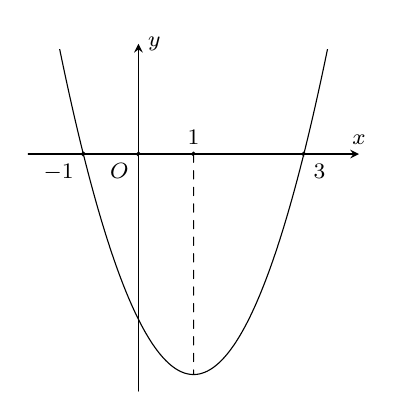
\begin{tikzpicture}[scale=0.7, font=\footnotesize, line join=round, line cap=round,>=stealth]
	\def\a{1} \def\b{1} \def\c{1} \def\d{-1} % Hệ số
	\def\xmin{-2} \def\xmax{4}
	\def\ymin{-4.3} \def\ymax{2}			
	\draw[->] (\xmin,0)--(\xmax,0) node [above]{$x$};
	\draw[->] (0,\ymin)--(0,\ymax) node [right]{$y$};
	\clip (\xmin+0.1,\ymin+0.1) rectangle (\xmax-0.1,\ymax-0.1);
	\draw[smooth,samples=300,domain=-1.5:3.5] plot(\x,{(\x)^2-2*(\x)-3});
	\draw[dashed] (1,0)--(1,-4)
	(-1,0) circle (1pt)node[below left]{$-1$}
	(3,0) circle (1pt)node[below right]{$3$}
	(1,0) circle (1pt)node[above]{$1$}
	(0,0) circle (1pt)node[below left]{$O$}
	;
	\end{tikzpicture}
	}
	\loigiai{
	Dựa vào đồ thị suy ra
	\[ f'(x) > 0\Leftrightarrow \hoac{&x <-1 \\ &x >3.}\]	
	Vì vậy, hàm số  đồng biến trên $(1;+\infty)$ và $(3;+\infty)$.
	}
\end{ex}
\begin{ex}%[Thi thử lần 1, THPT chuyên Thoại Ngọc Hầu - An Giang, năm 2020 - 2021]%[Trần Chiến, 12EX3]%[1D1B1-1]
	Tìm tập xác định $\mathscr{D}$ của hàm số $y= \dfrac{2020}{\sin x }$.
	\choice
	{$\mathscr{D} =\mathbb{R}$}
	{$\mathscr{D} = \mathbb{R} \setminus \{0\}$}
	{$\mathscr{D} = \mathbb{R} \setminus \left\{ \dfrac{\pi}{2}+k \pi , k \in \mathbb{Z} \right\}$}
	{\True $\mathscr{D}=\mathbb{R} \setminus \left\{ k \pi , k \in \mathbb{Z} \right\}$}
	\loigiai{
		Hàm số xác định khi $\sin x\ne 0 \Leftrightarrow x \ne k \pi , k \in \mathbb{Z}$.\\
		Vậy tập xác định của hàm số là $\mathscr{D}=\mathbb{R} \setminus \left\{ k \pi , k \in \mathbb{Z} \right\}$.
	}
\end{ex}
\begin{ex}%[Thi thử lần 1, THPT chuyên Thoại Ngọc Hầu - An Giang, năm 2020 - 2021]%[Trần Chiến, 12EX3]%[2D2B5-1]
	Nghiệm của phương trình $3^{2x-1}=27$ là
	\choice
	{$x=1$}
	{\True $x=2$}
	{$x=4$}
	{$x=5$}
	\loigiai{
	Ta có $3^{2x-1}=27 \Leftrightarrow 2x-1 =\log_3 27 \Leftrightarrow 2x-1=3 \Leftrightarrow x=2$.  
	}
\end{ex}
\begin{ex}%[Thi thử lần 1, THPT chuyên Thoại Ngọc Hầu - An Giang, năm 2020 - 2021]%[Trần Chiến, 12EX3]%[2D1Y4-1]
	Đồ thị hàm số $y=\dfrac{2x-1}{x+1}$ có bao nhiêu đường tiệm cận?
	\choice
	{$1$}
	{\True $2$}
	{$3$}
	{$4$}
	\loigiai{
	Ta có $\lim\limits_{x\to +\infty}y=2$ và $\lim\limits_{x\to -\infty}y=2$ nên đồ thị có 1 tiệm cận ngang là $y=2$.\\
	Ta có $\lim\limits_{x\to -1^+}y=-\infty$ và $\lim\limits_{x\to -1^-}y=+\infty$ nên đồ thị có 1 tiệm cận đứng là $x=-1$.\\
	Vậy đồ thị có 2 đường tiệm cận.
	}
\end{ex}
\begin{ex}%[Thi thử lần 1, THPT chuyên Thoại Ngọc Hầu - An Giang, năm 2020 - 2021]%[Trần Chiến, 12EX3]%[1D5B2-2]
	Viết phương trình tiếp tuyến của đồ thị hàm số $y=x^3 -2x+3$ tại điểm $M(1;2)$.
	\choice
	{$y=2x+2$}
	{$y=3x-2$}
	{\True $y=x+1$}
	{$y=2-x$}
	\loigiai{
	Ta có $y' = 3x^2-2$; $y'(1)=1$. \\
	Phương trình tiếp  tuyến của đồ thị hàm số $y=x^3 -2x+3$ tại điểm $M(1;2)$ là
	\[y= y'(1)(x-1)+2  \Leftrightarrow y=x+1.\]	
	}
\end{ex}

\begin{ex}%[Thi thử, Chuyên Thoại Ngọc Hầu, An Giang, lần 1 2021]%[Bùi Anh Tuấn, 12EX3]%[2D1B4-1]
	Đồ thị hàm số $y=\dfrac{\sqrt{x-7}}{x^2+3x-4}$ có bao nhiêu đường tiệm cận đứng?
	\choice
	{\True $0$}
	{$1$}
	{$2$}
	{$3$}
	\loigiai{ 
		Điều kiện xác định $\heva{& x-7\geq0 \\ & x^2+3x-4\ne 0}\Leftrightarrow \heva{& x\geq7 \\ &x\ne 1, x\ne 4}$ nên tập xác định $\mathscr{D}=[7;+\infty)$.\\
		Suy ra đồ thị hàm số không có đường tiệm cận đứng.	
	}
\end{ex}
\begin{ex}%[Thi thử lần 1, THPT chuyên Thoại Ngọc Hầu - An Giang, năm 2020 - 2021]%[Trần Chiến, 12EX3]%[1D3B3-4]
	Nếu các số $5+m; 7+2m; 17+m$ theo thứ tự lập thành cấp số cộng thì $m$ bằng bao nhiêu?
	\choice
	{$m=2$}
	{$m=3$}
	{\True $m=4$}
	{$m=5$}
	\loigiai{
		Ba số  $5+m; 7+2m; 17+m$ theo thứ tự lập thành cấp số cộng khi và chỉ khi
		\[2(7+2m) = 5+m+17+m \Leftrightarrow m= 4. \]
	}
\end{ex}
\begin{ex}%[Thi thử, Chuyên Thoại Ngọc Hầu, An Giang, lần 1 2021]%[Bùi Anh Tuấn, 12EX3]%[2D2K2-3]
	Hàm số $y=\sqrt[3]{x^2}$ có tất cả bao nhiêu điểm cực trị?
	\choice
	{$0$}
	{\True $1$}
	{$2$}
	{$3$}
	\loigiai{
		Tập xác định $\mathscr{D}=\mathbb{R}$. Ta có $y'=\dfrac{2}{3\sqrt[3]{x}},\,\forall x\neq 0$.\\
		Ta có $y'$ không xác định tại $x=0$ và $y'$ đổi dấu khi đi qua $x=0$. \\
		Vậy hàm số đạt cực trị tại $x=0$.
	}
\end{ex}

\begin{ex}%[Thi thử, Chuyên Thoại Ngọc Hầu, An Giang, lần 1 2021]%[Bùi Anh Tuấn, 12EX3]%[1D2B5-2]
	Gieo một con súc sắc cân đối và đồng chất hai lần. Tính xác suất để có ít nhất một lần xuất hiện mặt sáu chấm.
	\choice
	{\True $\dfrac{12}{36}$}
	{$\dfrac{11}{36}$}
	{$\dfrac{6}{36}$}
	{$\dfrac{8}{36}$}
	\loigiai{
		Ta có số phần tử của không gian mẫu bằng $6^2=36$.\\
		Gọi $A$ là biến cố xuất hiện ít nhất một lần mặt sáu chấm. Ta có số trường hợp thuận lợi cho biến cố $A$ bằng $11$, do $\Omega_{A}=\left\{(1;6),(2;6),(3;6),(4;6),(5;6),(6;1),(6;2),(6;3),(6;4),(6;5),(6;6)\right\}$.\\
		Vậy xác suất xảy ra biến cố $A$ bằng $\mathrm{P}(A)=\dfrac{11}{36}$.
		
	}
\end{ex}
\begin{ex}%[Đề giữa kì 1 THPT Chuyên Thoại Ngọc Hầu - An Giang - 21,EX3-24-Phan Anh]%[2D2B3-1]
	Cho $\log_ax=3$, $\log_bx=4$. Tính giá trị biểu thức $P=\log_{ab}x$.
	\choice
	{$P=\dfrac{1}{12}$}
	{$P=\dfrac{7}{12}$}
	{\True $P=\dfrac{12}{7}$}
	{$P=12$}
	\loigiai{Ta có \[\log_{ab}x=\dfrac{1}{\log_x(ab)}=\dfrac{1}{\log_xa+\log_xb}=\dfrac{1}{\dfrac{1}{\log_ax}+\dfrac{1}{\log_bx}}=\dfrac{1}{\dfrac{1}{3}+\dfrac{1}{4}}=\dfrac{12}{7}.\]
	}
\end{ex}
\begin{ex}%[Thi thử lần 1, THPT chuyên Thoại Ngọc Hầu - An Giang, năm 2020 - 2021]%[Trần Chiến, 12EX3]%[1D2K2-2]
	Có tất cả bao nhiêu số tự nhiên có $4$ chữ số khác nhau và khác $0$ mà trong mỗi số luôn có mặt hai chữ số chẵn và hai chữ số lẻ?
	\choice
	{$4!\mathrm{C}^1_4\mathrm{C}^1_5$}
	{$3!\mathrm{C}^2_3\mathrm{C}^2_5$}
	{\True $4!\mathrm{C}^2_4\mathrm{C}^2_5$}
	{$3!\mathrm{C}^2_4\mathrm{C}^2_5$}
	\loigiai{
		Số cách chọn $2$ số chẵn từ tập $\{2;4;\ldots, 8 \}$ là $\mathrm{C}^2_4$.\\
		Số cách chọn $2$ số lẻ từ tập $\{1;3;\ldots; 9\}$ là $\mathrm{C}^2_5$.\\
		Khi đó, số các số tự nhiên thỏa bài toán là $4!\mathrm{C}^2_4\mathrm{C}^2_5$.
	}
\end{ex}
\begin{ex}%[Thi thử lần 1, THPT chuyên Thoại Ngọc Hầu - An Giang, năm 2020 - 2021]%[Trần Chiến, 12EX3]%[1D2B3-2]
	Tìm hệ số của $x^{12}$ trong khai triển $(2x-x^2)^{10}$.
	\choice
	{$\mathrm{C}^8_{10}$}
	{\True $\mathrm{C}^2_{10} 2^8$}
	{$\mathrm{C}^2_{10}$}
	{$-\mathrm{C}^2_{10}2^8$}
	\loigiai{
		Số hạng tổng quát trong khai triển là 
		\[T= \mathrm{C}^k_{10} (2x)^{10-k} \cdot (-x^2)^k = \mathrm{C}^k_{10} (-1)^k\cdot 2^{10-k}\cdot x^{10+k},\] với $k \in \mathbb{N}$ và $k \le 10$.\\
		Số hạng chứa $x^{12}$ khi và chỉ khi $10+k =12 \Leftrightarrow k=2$ (thỏa điều kiện).\\
		Vậy hệ số của $x^{12}$ là $\mathrm{C}^2_{10}2^8$.
	}
\end{ex}
\begin{ex}%[Thi thử, Chuyên Thoại Ngọc Hầu, An Giang, lần 1 2021]%[Bùi Anh Tuấn, 12EX3]%[1H3B3-3]
	Cho hình chóp đều $S.ABCD$ có cạnh đáy bằng $2$, cạnh bên bằng $3$. Gọi $\varphi$ là góc giữa mặt bên và mặt đáy. Mệnh đề nào sau đây đúng?
	\choice
	{\True $\tan \varphi=\sqrt{7}$}
	{$\varphi=60^{\circ}$}
	{$\varphi=45^{\circ}$}
	{$\cos \varphi=\dfrac{\sqrt{2}}{3}$}
	\loigiai{
		\immini{
			Gọi $O$, $H$ lần lượt là trung điểm của  $AC$ và $CD$. \\
			Ta có $\heva{&OH\perp CD\\& SH\perp CD}\Rightarrow \left((SDC);(ABCD)\right)=\widehat{SHO}$.\\
			Trong $\triangle SHD$, ta có $SO^2=SD^2-OD^2=7\Rightarrow SO=\sqrt 7$.\\
			Trong $\triangle SOH$, ta có $\tan\varphi=\tan \widehat{SHO}=\dfrac{SO}{OH}=\dfrac{\sqrt{7}}{1}=\sqrt{7}$.
		}
		{\begin{tikzpicture}[scale=0.9,>=stealth, font=\footnotesize, line join=round, line cap=round]
				\tkzDefPoints{0/0/A,-1.9/-1.6/B,1.6/-1.6/C}
				\coordinate (D) at ($(A)+(C)-(B)$);
				\coordinate (O) at ($(A)!1/2!(C)$);
				\coordinate (S) at ($(O)+(0,3.5)$);
				\coordinate (H) at ($(C)!0.5!(D)$);
				\tkzDrawPolygon(S,B,C,D)
				\tkzDrawSegments(S,C S,H)
				\tkzDrawSegments[dashed](A,S A,B A,D A,C B,D S,O O,H)
				\tkzDrawPoints[fill=black,size=4](D,C,A,B,S,O,H)
				\tkzMarkRightAngles[size=0.16](A,O,B S,O,A S,O,B)
				\tkzMarkAngles[size=0.5cm,arc=l](S,H,O)	
				\tkzLabelAngles[pos=0.85,rotate=30](S,H,O){$\varphi$}
				\tkzLabelPoints[above](S)
				\tkzLabelPoints[below](A,C,O))
				\tkzLabelPoints[below left](B)
				\tkzLabelPoints[right](D,H)
		\end{tikzpicture}}
	}
\end{ex}	
\begin{ex}%[Thi thử, Chuyên Thoại Ngọc Hầu, An Giang, lần 1 2021]%[Bùi Anh Tuấn, 12EX3]%[2D1B5-1]
	\immini
	{
		Hàm số $ y=\dfrac{ax+b}{cx+d} $ với $ a > 0 $ có đồ thị như hình vẽ bên. Mệnh đề nào sau đây là đúng?
		%\choicew{0.45\textwidth}
		\choice
		{\True $ b>0,c>0,d<0 $}
		{$ b>0,c<0,d<0 $}
		{$ b<0,c<0,d<0 $}
		{$ b<0,c>0,d<0 $}
	}
	{
		\begin{tikzpicture}[scale=0.7, font=\footnotesize, line join=round, line cap=round, >=stealth]
			\def\xmin{-3}\def\xmax{4}\def\ymin{-3.0}\def\ymax{4.0}
			\draw[->] (\xmin,0)--(\xmax+0.2,0) node[below] {\footnotesize $x$};
			\draw[->] (0,\ymin)--(0,\ymax+0.2) node[left] {\footnotesize $y$};
			\fill (0,0)node[above right]{\footnotesize $O$}circle(2.5 pt);
			%\draw (0,0) node [above right] {\footnotesize $O$};
			\clip (\xmin,\ymin) rectangle (\xmax,\ymax);
			
			\draw[smooth,samples=200,domain=1.1:\xmax] plot (\x,{(1*(\x)+1)/(1*(\x)-1)});
			\draw[smooth,samples=200,domain=\xmin:0.9] plot (\x,{(1*(\x)+1)/(1*(\x)-1)});
			
			\draw[blue] (\xmin,1)--(\xmax,1);
			\draw[blue] (1,\ymin)--(1,\ymax);
		\end{tikzpicture}
	}
	
	\loigiai{
		\begin{itemize}		
			\item Cho $ y=0\Rightarrow x=-\dfrac{b}{a}<0\Rightarrow b>0 \ (a>0)$.
			\item Cho $ x=0\Rightarrow y=\dfrac{b}{d}<0\Rightarrow d<0 $.
			\item Đường tiệm cận đứng là $ x=-\dfrac{d}{c}>0\Rightarrow c>0 $.
		\end{itemize}
	}
\end{ex}

\begin{ex}%[Thi thử, Chuyên Thoại Ngọc Hầu, An Giang, lần 1 2021]%[Bùi Anh Tuấn, 12EX3]%[2D2B4-2]
	Cho hàm số $ f(x)=\ln 2020-\ln \left(\dfrac{x+1}{x}\right) $. Tính $ S=f'(1)+f'(2)+\ldots +f'(2020) $.
	\choice
	{$ S=2020 $}
	{$ S=2021 $}
	{$ S=\dfrac{2021}{2020} $}
	{\True $ S=\dfrac{2020}{2021} $}
	\loigiai{
		Ta có $ f'(x)=\dfrac{1}{x}-\dfrac{1}{x+1}$.
		\begin{eqnarray*}
			f'(1)&=&\dfrac{1}{1}-\dfrac{1}{2}\\
			f'(2)&=&\dfrac{1}{2}-\dfrac{1}{3}\\
			&& \cdots \\
			f'(2020)&=&\dfrac{1}{2020}-\dfrac{1}{2021}
		\end{eqnarray*}	
		Suy ra $ S=\dfrac{1}{1} -\dfrac{1}{2021}=\dfrac{2020}{2021} $.
	}
\end{ex}
\begin{ex}%[Thi thử, Chuyên Thoại Ngọc Hầu, An Giang, lần 1 2021]%[Bùi Anh Tuấn, 12EX3]%[2D1B5-3]
	\immini{Cho hàm số $y=f(x)$ liên tục trên $[-2;2]$ và có đồ thị là đường cong như hình vẽ bên. Hỏi phương trình $|f(x)-1|=1$ có bao nhiêu nghiệm phân biệt trên $[-2;2]$?
		\choice
		{$3$}
		{$4$}
		{\True $5$}
		{$6$}}{\begin{tikzpicture}[scale=.6, font=\footnotesize, line join=round, line cap=round, >=stealth, x=1.35cm, y=1cm]
			\def\xmin{-3}\def\xmax{3}\def\ymin{-4}\def\ymax{4}
			\draw[->] (\xmin-0.2,0)--(\xmax+0.2,0) node[below] {\footnotesize $x$};
			\draw[->] (0,\ymin-0.2)--(0,\ymax+0.2) node[right] {\footnotesize $y$};
			\draw (0,0) node [below left] {\footnotesize $O$};
			\fill (0,0) circle (2pt);
			\draw (-2.5,0) node [below ] {\footnotesize $-2$};
			\draw (2.15,0) node [below] {\footnotesize $2$};
			\draw (0,-3.85) node [left] {\footnotesize $-4$};
			\draw (0,3.65) node [left] {\footnotesize $4$};
			\draw (0,-1.9) node [left] {\footnotesize $-2$};
			\draw (0,1.9) node [right] {\footnotesize $2$};
			\foreach \x in {}\draw (\x,0.1)--(\x,-0.1) node [below] {\footnotesize $\x$};
			\foreach \y in {}\draw (0.1,\y)--(-0.1,\y) node [left] {\footnotesize $\y$};
			\clip (\xmin,\ymin) rectangle (\xmax,\ymax);
			\draw[smooth,samples=200,domain=\xmin:\xmax] plot (\x,{1*((\x)^3)+0*((\x)^2)+-3*(\x)+0});
			\draw[dashed] (0.0,0)--(0.0,0.0)--(0,0.0);\fill (0.0,0.0) circle (1pt);
			\draw[dashed] (-2.15,0)--(-2.15,-3.5)--(0,-3.5);\fill (-2.15,-3.5) circle (1pt);
			\draw[dashed] (2.15,0)--(2.15,3.5)--(0,3.5);\fill (2.15,3.5) circle (1pt);
			\draw[dashed] (1.0,-2.0)--(0,-2.0);\fill (1.0,-2.0) circle (1pt);
			\draw[dashed] (-1.0,2.0)--(0,2.0);\fill (-1.0,2.0) circle (1pt);
	\end{tikzpicture}}
	\loigiai{
		Xét phương trình $|f(x)-1|=1\Leftrightarrow \hoac{&f(x)-1=1\\&f(x)-1=-1}\Leftrightarrow \hoac{&f(x)=0\\&f(x)=2.}$
		\begin{itemize}
			\item Trường hợp 1: Phương trình $f(x)=0$ có $3$ nghiệm $x_1,\ x_2,\ x_3 \in [-2;2]$.
			\item Trường hợp 2: Phương trình $f(x)=2$ có $2$ nghiệm $x_4,\ x_5\in [-2;2]$.   
		\end{itemize}
		Dễ thấy các nghiệm này không trùng nhau.\\
		Vậy phương trình $|f(x)-1|=1$ có $5$ nghiệm phân biệt thuộc đoạn $[-2;2]$.
	}
\end{ex}

\begin{ex}%[Đề giữa kì 1 THPT Chuyên Thoại Ngọc Hầu - An Giang - 21,EX3-24-Phan Anh]%[2H1B3-2]
	Cho hình lăng trụ $ABC.A'B'C'$ có đáy $ABC$ là tam giác vuông cân tại $B$ và $AC=2a$. Hình chiếu vuông góc của $A'$ trên mặt phẳng $(ABC)$ là trung điểm $H$ của cạnh $AB$ và $A'A=a\sqrt{2}$. Thể tích $V$ của khối lăng trụ đã cho bằng
	\choice
	{$V=a^3\sqrt{3}$}
	{$V=2a^3\sqrt{2}$}
	{\True $V=\dfrac{a^3\sqrt{6}}{2}$}
	{$V=\dfrac{a^3\sqrt{6}}{6}$}
	\loigiai{\immini{Ta có $ABC$ là tam giác vuông cân tại $B$ nên
			$$AB=BC=\dfrac{AC}{\sqrt{2}}=a\sqrt{2}.$$
			Tam giác $A'AH$ vuông tại $H$ có 
			$$A'H=\sqrt{AA'^2-AH^2}=\sqrt{2a^2-\dfrac{2a^2}{4}}=\dfrac{a\sqrt{6}}{2}.$$
			Thể tích của khối lăng trụ là
			$$V=A'H\cdot S_{ABC}=\dfrac{a\sqrt{6}}{2}\cdot\dfrac{1}{2}\cdot\left(a\sqrt{2}\right)^2=\dfrac{a^3\sqrt{6}}{2}.$$}
		{\begin{tikzpicture}[scale=0.6,font=\footnotesize]
				\tkzDefPoints{0/0/A, 3/-1.8/B, 7/0/C}
				\coordinate (H) at ($(A)!0.5!(B)$);
				\coordinate (A') at ($(H)+(0,6)$);
				\coordinate (B') at ($(A')+(B)-(A)$);
				\coordinate (C') at ($(A')+(C)-(A)$);
				\tkzDrawPoints[fill=black](A,B,C,A',B',C',H)
				\tkzDrawSegments(A,B B,C A,A' B,B' C,C' A',B' B',C' C',A' A',H)
				\tkzDrawSegments[dashed](A,C)
				\tkzLabelPoints[below](B)
				\tkzLabelPoints[below left](A,H)
				\tkzLabelPoints[below right](C)
				\tkzLabelPoints[above left](A')
				\tkzLabelPoints[above right](C')
				\tkzLabelPoints[above](B')
				\tkzMarkRightAngle(C,B,A)
	\end{tikzpicture}}}
\end{ex}
\begin{ex}%[Thi thử lần 1, THPT chuyên Thoại Ngọc Hầu - An Giang, năm 2020 - 2021]%[Trần Chiến, 12EX3]%[2D2B3-1]
	Cho hai số thực dương $m,n$ và $(n\ne 1)$ thỏa mãn $\dfrac{\log_7 m\cdot \log_2 7}{\log_2 10 -1}=3+\dfrac{1}{\log_n 5}$. Khẳng định nào sau đây là đúng?
	\choice
	{$m=15n$}
	{$m=25n$}
	{\True $m=125n$}
	{$m\cdot n=125$}
	\loigiai{
		Ta có
		\begin{eqnarray*}
			\dfrac{\log_7 m\cdot \log_2 7}{\log_2 10 -1}=3+\dfrac{1}{\log_n 5} &\Leftrightarrow& \dfrac{\log_2 m}{\log_2 5} =3+\log_5 n \\
			&\Leftrightarrow& \log_5m = \log_5 125n \\
			&\Leftrightarrow& m=125n.	
		\end{eqnarray*}
	}
\end{ex}
\begin{ex}%[Đề giữa kì 1 THPT Chuyên Thoại Ngọc Hầu - An Giang - 21,EX3-24-Phan Anh]%[2H1K3-3]
	Cho tứ diện $ABCD$ có $AB$, $AC$, $AD$ đôi một vuông góc nhau và $AB=6a$, $AC=9a$, $AD=3a$. Gọi $M$, $N$, $P$ lần lượt là trọng tâm của các tam giác $ABC$, $ACD$, $ADB$. Thể tích $V$ của khối tứ diện $AMNP$ bằng
	\choice
	{\True $V=2a^3$}
	{$V=4a^3$}
	{$V=6a^3$}
	{$V=8a^3$}
	\loigiai{\immini{Gọi $I$, $J$, $K$ lần lượt là trung điểm của $BC$, $CD$, $BD$.\\
			Ta có $\dfrac{V_{A.MNP}}{V_{A.IJK}}=\dfrac{AM}{AI}\cdot\dfrac{AN}{AJ}\cdot\dfrac{AP}{AK}=\left(\dfrac{2}{3}\right)^3=\dfrac{8}{27}$.\\
			Do $I$, $J$, $K$ là trung điểm nên $S_{IJK}=\dfrac{1}{4}S_{BCD}$.\\
			Vậy ta có $V_{A.IJK}=\dfrac{1}{4}V_{A.BCD}$.\\
			Thể tích khối $A.MNP$ là
			$$V=\dfrac{8}{27}\cdot\dfrac{1}{4}\cdot\dfrac{1}{6}\cdot AB\cdot AC\cdot AD=2a^3.$$}
		{\begin{tikzpicture}[scale=0.75]
				\tkzDefPoints{0/0/A,0/5.5/B,6.5/0/D,-2/-2/C}
				\coordinate (I) at ($(B)!0.5!(C)$);
				\coordinate (M) at ($(A)!{2/3}!(I)$);
				\coordinate (J) at ($(D)!0.5!(C)$);
				\coordinate (N) at ($(A)!{2/3}!(J)$);
				\coordinate (K) at ($(B)!0.5!(D)$);
				\coordinate (P) at ($(A)!{2/3}!(K)$);
				\tkzDrawPoints[fill=black](A,B,C,D,M,N,P,I,J,K)
				\tkzDrawSegments(B,C C,D D,B I,J J,K K,I)
				\tkzDrawSegments[dashed](A,B A,C A,D A,I A,J A,K M,N M,P N,P)
				\tkzLabelPoints[left](A,I)
				\tkzLabelPoints[above](B)
				\tkzLabelPoints[below](M)
				\tkzLabelPoints[below left](C,N)
				\tkzLabelPoints[above right](D,K)
				\tkzLabelPoints[below right](J,P)
	\end{tikzpicture}}}
\end{ex}
\begin{ex}%[Thi thử lần 1, THPT chuyên Thoại Ngọc Hầu - An Giang, năm 2020 - 2021]%[Trần Chiến, 12EX3]%[2D1K1-3]
	Tính tổng các giá trị nguyên của tham số $m$ thuộc đoạn $[-20;20]$ để hàm số $y=\dfrac{\sin x+m}{\sin x-1}$ nghịch biến trên khoảng $\left(\dfrac{\pi}{2}; \pi \right)$.
	\choice
	{$209$}
	{$207$}
	{\True $-209$}
	{$-210$}
	\loigiai{
		Ta có $y' = \dfrac{-\cos x(1+m)}{(\sin x-1)^2},\,\forall x\neq \dfrac{\pi}{2}+k2\pi\ (k\in\mathbb{Z})$.
		\\
		Hàm số  nghịch biến trên khoảng $\left(\dfrac{\pi}{2}; \pi \right) \Leftrightarrow y' \le 0 ,\,\forall x \in \left(\dfrac{\pi}{2}; \pi \right)$. \hfill $(*)$\\
		Vì $-\cos x >0,\, \forall x \in \left(\dfrac{\pi}{2}; \pi \right)$ nên $(*)$ tương đương với
		\[ \heva{& 1+m <0 \\ & \sin x \ne 1, \ \forall x \in \left(\dfrac{\pi}{2}; \pi \right) \ (\text{luôn đúng})} \Leftrightarrow m<-1.\]
		Mà $m$ nguyên thuộc đoạn $[-20;20]$ nên ta có $m\in\{-20,-19,\ldots,-2\}$.\\
		Vậy tổng các giá trị của $m$ thỏa bài toán là $-20+(-19)+\ldots + -2 =-209$.	
	}
\end{ex}
\begin{ex}%[Thi thử, Chuyên Thoại Ngọc Hầu, An Giang, lần 1 2021]%[Bùi Anh Tuấn, 12EX3]%[2H1B3-3] 
	Cho hình chóp $S.ABCD$ có đáy $ABCD$ là hình bình hành và có thể tích bằng $48$. Gọi $M,N$ lần lượt là điểm thuộc các cạnh $AB, CD$ sao cho $MA=MB, NC=2ND$. Thể tích của khối chóp $S.MBCN$ bằng
	\choice
	{$8$}
	{$20$}
	{\True $28$}
	{$40$}
	\loigiai{
		\begin{center}
			\begin{tikzpicture}[scale=1, font=\footnotesize, line join=round, line cap=round, >=stealth]
				\tkzDefPoints{0/0/A,-1.5/-1.6/B,2.5/-1.6/C}
				\coordinate (D) at ($(A)+(C)-(B)$);
				\coordinate (S) at ($(A)+(0,3.5)$);
				\coordinate (M) at ($(A)!1/2!(B)$);
				\coordinate (N) at ($(C)!2/3!(D)$);
				\tkzDrawPolygon(S,B,C,D)
				\tkzDrawSegments(S,C S,N)
				\tkzDrawSegments[dashed](A,S A,B A,D S,M M,N M,C)
				\tkzDrawPoints[fill=black,size=4](D,C,A,B,S,M,N)
				\tkzLabelPoints[above](S)
				\tkzLabelPoints[below](B,C,M)
				\tkzLabelPoints[left](A)
				\tkzLabelPoints[right](D,N)
			\end{tikzpicture}
		\end{center}
		Ta có 
		\begin{itemize}
			\item $\dfrac{V_{B.MSC}}{V_{B.ASC}}=\dfrac{BM}{BA}=\dfrac{1}{2}\Rightarrow V_{B.MSC}=\dfrac{1}{2} \cdot V_{B.ASC}=\dfrac{1}{4} \cdot V_{S.ABCD}$.
			\item $\dfrac{V_{C.MSN}}{V_{C.MSD}}=\dfrac{CN}{CD}=\dfrac{2}{3}\Rightarrow V_{C.MSN}=\dfrac{2}{3} \cdot V_{C.MSD}=\dfrac{1}{3} \cdot V_{S.ABCD}$.
		\end{itemize}
		Do đó 
		$$ V_{S.MBCN}=V_{B.MSC}+V_{C.MSN}=\dfrac{1}{4} \cdot V_{S.ABCD}+\dfrac{1}{3} \cdot V_{S.ABCD}=\dfrac{7}{12} \cdot V_{S.ABCD}=\dfrac{7}{12}\cdot 48=28.$$
	}
\end{ex}
\begin{ex}%[Thi thử lần 1, THPT chuyên Thoại Ngọc Hầu - An Giang, năm 2020 - 2021]%[Trần Chiến, 12EX3]%[2H1K3-4]
	Cho hình chóp $S.ABCD$ có đáy $ABCD$ là hình chữ nhật với $AB=a$, $AD=2a$. Cạnh bên $SA=2a$ và vuông góc với đáy. Gọi $M, N$ lần lượt là trung điểm của $SB$ và $SD$. Tính khoảng cách $d$ từ $S$ đến mặt phẳng $(AMN)$.
	\choice
	{\True $d=\dfrac{a\sqrt{6}}{3}$}
	{$d=2a$}
	{$d=\dfrac{3a}{2}$}
	{$d=a\sqrt{5}$}
	\loigiai{
		\immini{
			Ta có 
			\begin{eqnarray*}
				V_{S.AMN}&=&\dfrac{SM}{SB}\cdot \dfrac{SN}{SD} \cdot  V_{S.ABD}\\ &=&\dfrac{1}{4}\left(\dfrac{1}{2}V_{S.ABCD}\right)=\dfrac{1}{8}V_{S.ABCD} \\
				&=& \dfrac{1}{8} \cdot \dfrac{1}{3}\cdot SA\cdot AB \cdot AD = \dfrac{a^3}{6}.
			\end{eqnarray*}
			Do $\Delta SAB$ vuông tại $A$ nên \[AM =\dfrac{1}{2}SB=\dfrac{1}{2}\sqrt{SA^2+AB^2} =\dfrac{a\sqrt{5}}{2}.\]
		}{
			\begin{tikzpicture}[scale=1, font=\footnotesize, line join=round, line cap=round,>=stealth]
				\tkzDefPoints{0/0/A,5/0/D,-1.5/-1.5/B}
				\coordinate (C) at ($(D)-(A)+(B)$);
				\coordinate (S) at ($(A)+(0,4)$);
				\coordinate (M) at ($(S)!0.5!(B)$);
				\coordinate (N) at ($(S)!0.5!(D)$);
				\tkzDrawSegments(S,B S,C S,D B,C C,D)
				\tkzDrawSegments[dashed](S,A A,B A,D A,M A,N M,N B,D)
				\tkzLabelPoints[above](S)
				\tkzLabelPoints[below left](B)
				\tkzLabelPoints[below right](C,D)
				\tkzLabelPoints[below](A)
				\tkzLabelPoints[above left](M)
				\tkzLabelPoints[above right](N)
				\tkzDrawPoints(S,A,B,C,D,M,N)
			\end{tikzpicture}
		}
		\noindent
		Do $\Delta SAD$ vuông tại $A$ nên $AN =\dfrac{1}{2}SD=\dfrac{1}{2}\sqrt{SA^2+AD^2} =a\sqrt{2}$.\\
		Do $MN$ là đường trung bình của $\Delta SBD$ nên $MN=\dfrac{1}{2}BD= \dfrac{a\sqrt{5}}{2}$.\\
		Tính được nửa chu vi $\Delta AMN$ là $p=\dfrac{AM+AN+MN}{2}=\dfrac{\sqrt{2}+\sqrt{5}}{2}a$.\\
		Suy ra $S_{\Delta AMN} =\sqrt{p(p-AM)(p-AM)(p-MN)}=\dfrac{\sqrt{6}a^2}{4}$.\\
		Khi đó $d= \mathrm{d}(S, (AMN)) =\dfrac{3V_{S.AMN}}{S_{\Delta AMN}} = \dfrac{a\sqrt{6}}{3}$.
	}
\end{ex}
\begin{ex}%[Thi thử, Chuyên Thoại Ngọc Hầu, An Giang, lần 1 2021]%[Bùi Anh Tuấn, 12EX3]%[2H1K3-3]
	Cho hình lập phương $ABCD.A'B'C'D'$, gọi $I$ là trung điểm của cạnh $BB'$. Mặt phẳng $(DIC')$ chia hình lập phương thành hai phần. Tính tỉ số thể tích giữa phần bé và phần lớn. 
	\choice
	{\True $\dfrac{7}{17}$}
	{$\dfrac{1}{3}$}
	{$\dfrac{1}{2}$}
	{$\dfrac{1}{7}$}
	\loigiai{ 
		\immini{Giả sử $AB=a$. Gọi $J$ là giao điểm của $C'I$ và $BC$, $K$ là giao điểm của $DJ$ và $AB$.\\
			Mặt phẳng $(DIC')$ chia khối lập phương $ABCD.A'B'C'D'$ thành hai khối đa diện $C'CDKBI$ và khối đa diện $A'B'C'D'DIKA$.\\
			Do $BI\parallel CC'$ mà $I$ là trung điểm của $BB'$ nên $B$ là trung điểm của $JC$ hay $JB=BC=a$.\\ 
			Tương tự $K$ là trung điểm của $AB$ do đó $BK=KA=\dfrac{a}{2}$.\\
		}
		{\begin{tikzpicture}[scale=1]
				\tkzDefPoints{0/0/A, 1/1/B, 3/0/D, 1/4/z} 
				\coordinate (C) at ($(B)+(D)-(A)$);
				\tkzDefSquare(B,C) \tkzGetPoints{C'}{B'} 
				\tkzDefSquare(A,D) \tkzGetPoints{D'}{A'} 
				\tkzDefMidPoint(B,B')
				\tkzGetPoint{I}
				\tkzInterLL(C',I)(B,C)
				\tkzGetPoint{J}
				\tkzInterLL(C',I)(A,A')
				\tkzGetPoint{M}
				\tkzInterLL(D,J)(A,B)
				\tkzGetPoint{K}
				\tkzInterLL(D,J)(A,A')
				\tkzGetPoint{N}
				\tkzDrawSegments(A',B' B',C' C',D' D',A' A',A A,D D,D' D,C C,C' D,C' M,J N,J)
				\tkzDrawSegments[dashed](A,B B,C B,B' C',M C,J D,N D,I K,I)
				\tkzLabelPoints[above](A',D',C',B')
				\tkzLabelPoints[below](A,C,D,K)
				\tkzLabelPoints[above right](I,B)
				\tkzLabelPoints[left](J)
				\fill (A)circle(1.5pt) (B)circle(1.5pt) (C)circle(1.5pt) (D)circle(1.5pt) (A')circle(1.5pt) (B')circle(1.5pt) (C')circle(1.5pt) (D')circle(1.5pt) (I)circle(1.5pt) (J)circle(1.5pt) (K)circle(1.5pt);
		\end{tikzpicture}}
		\noindent Ta có $V_{J.DCC'}=\dfrac{1}{6}JC\cdot CD\cdot CC'=\dfrac{a^3}{3}$ 
		và $V_{J.KBI}=\dfrac{1}{6}JB\cdot BI \cdot BK=\dfrac{a^3}{24}$.\\
		Do đó $V_{C'CDKBI}=V_{J.DCC'}-V_{J.KBI}=\dfrac{a^3}{3}-\dfrac{a^3}{24}=\dfrac{7a^3}{24}.$\\
		Thể tích khối lập phương $ABCD.A'B'C'D'$ bằng $a^3.$\\
		Ta có
		\begin{eqnarray*}
			&&V_{ABCD.A'B'C'D'}=V_{C'CDKBI}+V_{A'B'C'D'DIKA}\\
			&\Rightarrow& V_{A'B'C'D'DIKA}=V_{ABCD.A'B'C'D'}-V_{C'CDKBI}=\dfrac{17a^3}{24}\\
			&\Rightarrow& \dfrac{V_{C'CDKBI}}{V_{A'B'C'D'DIKA}}=\dfrac{7}{17}.
		\end{eqnarray*}
	}
\end{ex}
\begin{ex}%[Đề giữa kì 1 THPT Chuyên Thoại Ngọc Hầu - An Giang - 21,EX3-24-Phan Anh]%[2D1G5-3]
	\immini{Cho hàm số bậc ba $y=f(x)$ có đồ thị là đường cong như hình vẽ bên. Hỏi phương trình $f(xf(x))-2=0$ có bao nhiêu nghiệm phân biệt?
		\choice
		{$3$}
		{$4$}
		{$5$}
		{\True $6$}}
	{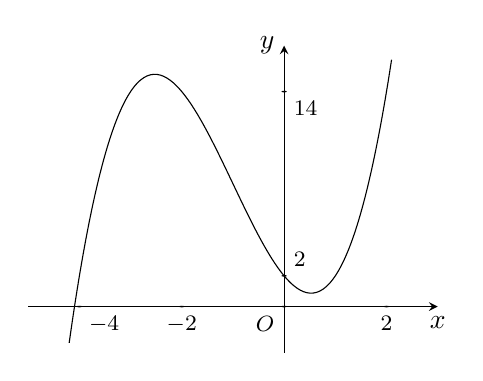
\begin{tikzpicture}[>=stealth,scale=0.65,yscale=0.3]
			%		\draw[thin,color=gray!20](-5,-3)grid(3,17);
			\draw[->](-5,0)--(3,0)node[below]{$x$};
			\draw[->](0,-3)--(0,17)node[left]{$y$};
			\draw[smooth, samples=100, domain=-4.2:2.1]plot(\x,{(\x)*(\x+4)*(\x-1)+2});
			\fill (0,0)node[below left]{\footnotesize{$O$}}circle(1.5pt) (-2,0)node[below]{\footnotesize{$-2$}}circle(1.5pt) (2,0)node[below]{\footnotesize{$2$}}circle(1.5pt) (-4,0)node[below right]{\footnotesize{$-4$}}circle(1.5pt) (0,2)node[above right]{\footnotesize{$2$}}circle(1.5pt) (0,14)node[below right]{\footnotesize{$14$}}circle(1.5pt);
	\end{tikzpicture}}
	\loigiai{
		Ta có \[f(xf(x))-2=0\Leftrightarrow f(xf(x))=2\Leftrightarrow\hoac{&xf(x)=\alpha\in(0;2)\\&xf(x)=0\\&xf(x)=\beta\in(-\infty,-2)}\Leftrightarrow\hoac{&f(x)=\dfrac{\alpha}{x}\\&x=0\\&f(x)=0\\&f(x)=\dfrac{\beta}{x}.}\]
		Xét hàm số $y=\dfrac{\alpha}{x}$ ta có $y'=-\dfrac{\alpha}{x^2}<0$, $\forall x\ne0$, nên có bảng biến thiên như hình vẽ.
		\begin{center}
			
\begin{tikzpicture}
				\tkzTabInit[nocadre=false, lgt=1.2, espcl=3.5, deltacl=0.6]
				{$x$/0.7, $y'$/0.7, $y$/2.3}
				{$-\infty$,$0$,$+\infty$}
				\tkzTabLine{,-,d,-,}
				\tkzTabVar{+/$0$,-D+/$-\infty$/$+\infty$,-/$0$}
			\end{tikzpicture}
		\end{center}
		Kết hợp đồ thị hàm số $y=f(x)$, phương trình $f(x)=\dfrac{\alpha}{x}$ có $2$ nghiệm.\\
		Xét hàm số $y=\dfrac{\beta}{x}$ ta có $y'=-\dfrac{\beta}{x^2}>0$, $\forall x\ne0$, nên có bảng biến thiên như hình vẽ.
		\begin{center}
			
\begin{tikzpicture}
				\tkzTabInit[nocadre=false, lgt=1.2, espcl=3.5, deltacl=0.6]
				{$x$/0.7, $y'$/0.7, $y$/2.3}
				{$-\infty$,$0$,$+\infty$}
				\tkzTabLine{,+,d,+,}
				\tkzTabVar{-/$0$,+D-/$+\infty$/$-\infty$,+/$0$}
			\end{tikzpicture}
		\end{center}
		Kết hợp đồ thị hàm số $y=f(x)$, phương trình $f(x)=\dfrac{\beta}{x}$ có $2$ nghiệm.\\
		Mặt khác $f(x)=0$ cũng có $1$ nghiệm duy nhất.\\
		Nhận thấy các nghiệm này không trùng nhau và khác $0$ nên suy ra phương trình $f(xf(x))-2=0$ có $6$ nghiệm.
	}
\end{ex}
\begin{ex}%[Thi thử, Chuyên Thoại Ngọc Hầu, An Giang, lần 1 2021]%[Bùi Anh Tuấn, 12EX3]%[2D1K2-6]
	\immini{Cho hàm số $y=f(x)$ là hàm đa thức bậc bốn có đồ thị như hình vẽ bên. Có bao nhiêu giá trị của tham số $m$ thuộc đoạn $[-12;12]$ để hàm số $g(x)=\left|2f(x-1)+m\right|$ có $5$ điểm cực trị?
		\choice
		{$13$}
		{$14$}
		{\True $15$}
		{$12$}}
	{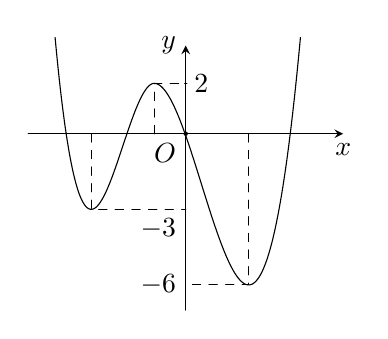
\begin{tikzpicture}[scale=0.4,line join=round,x=1cm, y=0.8cm, line cap=round,>=stealth]
			\draw[->] (-5,0)--(5,0) node[below] {$x$};
			\draw[->] (0,-7)--(0,3.5) node[left] {$y$};
			\fill (0,0)node[below left]{$O$}circle(2 pt);
			\foreach \y in {2}
			\draw[thin] (1pt,\y)--(-1pt,\y) node [right] {$\y$};
			\draw (0,-3) node[below left]{$-3$};
			\draw (0,-6) node[left]{$-6$};
			\draw[dashed](-3,0)--(-3,-3)--(0,-3);
			\draw[dashed](-1,0)--(-1,2)--(0,2);
			\draw[dashed](2,0)--(2,-6)--(0,-6);
			\clip (-5,-7) rectangle (5,3.8);
			\draw[samples=200,domain=-4.5:-1,smooth,variable=\x] plot (\x,{-1.25*((\x)^3)-7.5*((\x)^2)-11.25*(\x)-3});
			\draw[samples=200,domain=-1:4,smooth,variable=\x] plot (\x,{0.59259*((\x)^3)-0.88888*((\x)^2)-3.555555*(\x)-0.074});
		\end{tikzpicture}
	}
	\loigiai{
		Ta có
		\begin{eqnarray*}			
			g(x)&=&\left|2f(x-1)+m\right|=\sqrt{(2f(x-1)+m)^2}\\
			\Rightarrow g'(x)&=&\dfrac{2f'(x-1)\cdot (2f(x-1)+m)}{\sqrt{(2f(x-1)+m)^2}}.
		\end{eqnarray*}
		Xét $g'(x)=0\Leftrightarrow \hoac{& f'(x-1)=0\\ & 2f(x-1)+m=0}\Leftrightarrow \hoac{& f'(x-1)=0& (1)\\& f(x-1)=\dfrac{-m}{2}.& (2)}$\\
		Do đồ thị hàm số $y=f(x)$ có $3$ điểm cực trị $x=a$, $x=b$, $x=c$ nên phương trình $(1)$ có $3$ nghiệm phân biệt $x=a+1$, $x=b+1$, $x=c+1$.\\
		Do đó để hàm số $g(x)$ có $5$ điểm cực trị thì phương trình $(2)$ phải có $2$ nghiệm phân biệt không trùng với nghiệm của phương trình $ (1) $, hoặc phương trình $(2)$ có $3$ nghiệm phân biệt, trong đó $1$ nghiệm trùng với nghiệm của phương trình $ (1) $.\\
		Đồ thị hàm số $y=f(x-1)$ có được bằng cách tịnh tiến đồ thị hàm số $y=f(x)$ sang phải $1$ đơn vị. Khi đó,
		\[\hoac{& -\dfrac{m}{2}\geq 2\\& -6< -\dfrac{m}{2}\leq -3}\Leftrightarrow \hoac{ & m\leq -4\\ & 6\leq m<12.}\]
		Do $m$ nguyên và thuộc đoạn $[-12;12]$ nên $m\in \{-12;-11;\ldots;-5;-4\}$ hoặc $m\in \{6;7;8;\ldots;11\}$ do đó có tất cả $9+6=15$ giá trị cần tìm.
		
	}
\end{ex}
\begin{ex}%[Thi thử, Chuyên Thoại Ngọc Hầu, An Giang, lần 1 2021]%[Bùi Anh Tuấn, 12EX3]%[2D2G5-3]
	Cho các số thực $x$, $y$ thỏa mãn $4^{x^2+4y^2}-2^{x^2+4y^2+1}=2^{3-x^2-4y^2}-4^{2-x^2-4y^2}$. Gọi $m$, $M$ lần lượt là giá trị nhỏ nhất và lớn nhất của $P=\dfrac{x-2y-1}{x+y+4}$. Tổng $m+M$ bằng
	\choice
	{\True $-\dfrac{36}{59}$}
	{$-\dfrac{18}{59}$}
	{$\dfrac{18}{59}$}
	{$\dfrac{36}{59}$}
	\loigiai{
		Phương trình đã cho tương đương với $4^{x^2+4y^2}+\dfrac{16}{4^{x^2+4y^2}}=2\left(2^{x^2+4y^2}+\dfrac{4}{2^{x^2+4y^2}}\right)$.\quad\quad $(*)$\\
		Đặt $t=2^{x^2+4y^2}+\dfrac{4}{2^{x^2+4y^2}}$, $t \geq 2$. Suy ra $t^2=4^{x^2+4y^2}+\dfrac{15}{4^{x^2+4y^2}}+8$.\\
		Khi đó $(*)$ tương đương với $t^2-8=2t \Leftrightarrow \hoac{&t=4&\text{(nhận)}\\&t=-2.&\text{(loại)}}$\\
		Với $t=4\Leftrightarrow 2^{x^2+4y^2}+\dfrac{4}{2^{x^2+4y^2}}=4$.\quad\quad $(**)$\\
		Đặt $a=2^{x^2+4y^2}$, $a>0$.\\
		Khi đó, phương trình $(**)$ tương đương với 
		\begin{eqnarray*}
			&&a+\dfrac{4}{a}=4\\
			&\Leftrightarrow&a^2-4a+4=0\\
			&\Leftrightarrow& a=2.
		\end{eqnarray*}
		Với $a=2\Rightarrow 2^{x^2+4y^2}=2 \Leftrightarrow x^2+4y^2=1$.\\
		Đặt $\heva{&x=\sin t\\&2y=\cos t.}$\quad\quad $(1)$\\
		Mặt khác  $P=\dfrac{x-2y-1}{x+y+4}\Leftrightarrow (P-1)x+(P+2)y=-1-4P$.\quad\quad $(2)$\\
		Từ $(1)$ và $(2)$, ta có phương trình 
		\begin{eqnarray*}
			&&(P-1) \sin t+\left(\dfrac{P+2}{2}\right)\cos t=-1-4P\\
			&\Leftrightarrow& (2P-2)\sin t+ (P+2)\cos t=-2-8P. \quad\quad (3)
		\end{eqnarray*}	
		Để phương trình $(3)$ có nghiệm thì 
		\begin{eqnarray*}
			&&(2P-2)^2+(P+2)^2 \geq (-2-8P)^2\\
			&\Leftrightarrow& 59P^2+36P-4 \leq 0\\
			&\Leftrightarrow&\dfrac{-18-4\sqrt{35}}{59} \leq P \leq \dfrac{-18+4\sqrt{35}}{59}
		\end{eqnarray*}	
		Vậy $\heva{&m=\dfrac{-18-4\sqrt{35}}{59}\\&M=\dfrac{-18+4\sqrt{35}}{59}}\Rightarrow m+M=-\dfrac{36}{59}$.
	}
\end{ex}

\Closesolutionfile{ans}
\begin{indapan}{10}
	{ans/ans-2-GHK1-24-ChuyenThoaiNgocHau-AnGiang-21}
\end{indapan}